Moduł serwera służący do przesyłu danych między aplikacją a klientem złożony jest z dwóch głównych części:
\begin{enumerate}
\item komunikacji z aplikacją,
\item komunikacji z klientem.
\end{enumerate}
Komunikują się one przesyłając dane w formacie \emph{JSON}. \emph{Event Dispather} posiada jedno wejście przyjmujące opis zdarzeń zaistniałych po stronie klienta. \emph{Event Filter} posiada dwa wyjścia, którymi przekazuje dane do serwera \emph{WebSocket}, który następnie przekazuje je klientowi. Jedno wyjście przekazuje opis graficznych elementów interfejsu. Drugie natomiast obrazy w formacie \emph{PNG}. Powodem, dla którego postanowiono oddzielić przesyłanie obrazów od przesyłania opisu w formasie \emph{JSON} jest zbyt duży narzut na rozmiar pliku graficznego po konwersji do postaci tekstowej. \emph{Serwer WebSocket} nie wysyła więc obrazów bezpośrednio do klienta. Przesyła mu jedynie indentyfikator obrazu, a same dane są przekazywane do \emph{serwera obrazów}, który stanowi bufor dla plików graficznych. Bufor ten jest na bieżąco opróżniany, w momencie gdy klient zdecyduje się pobrać dany obraz.

\begin{figure}[H]
\centering
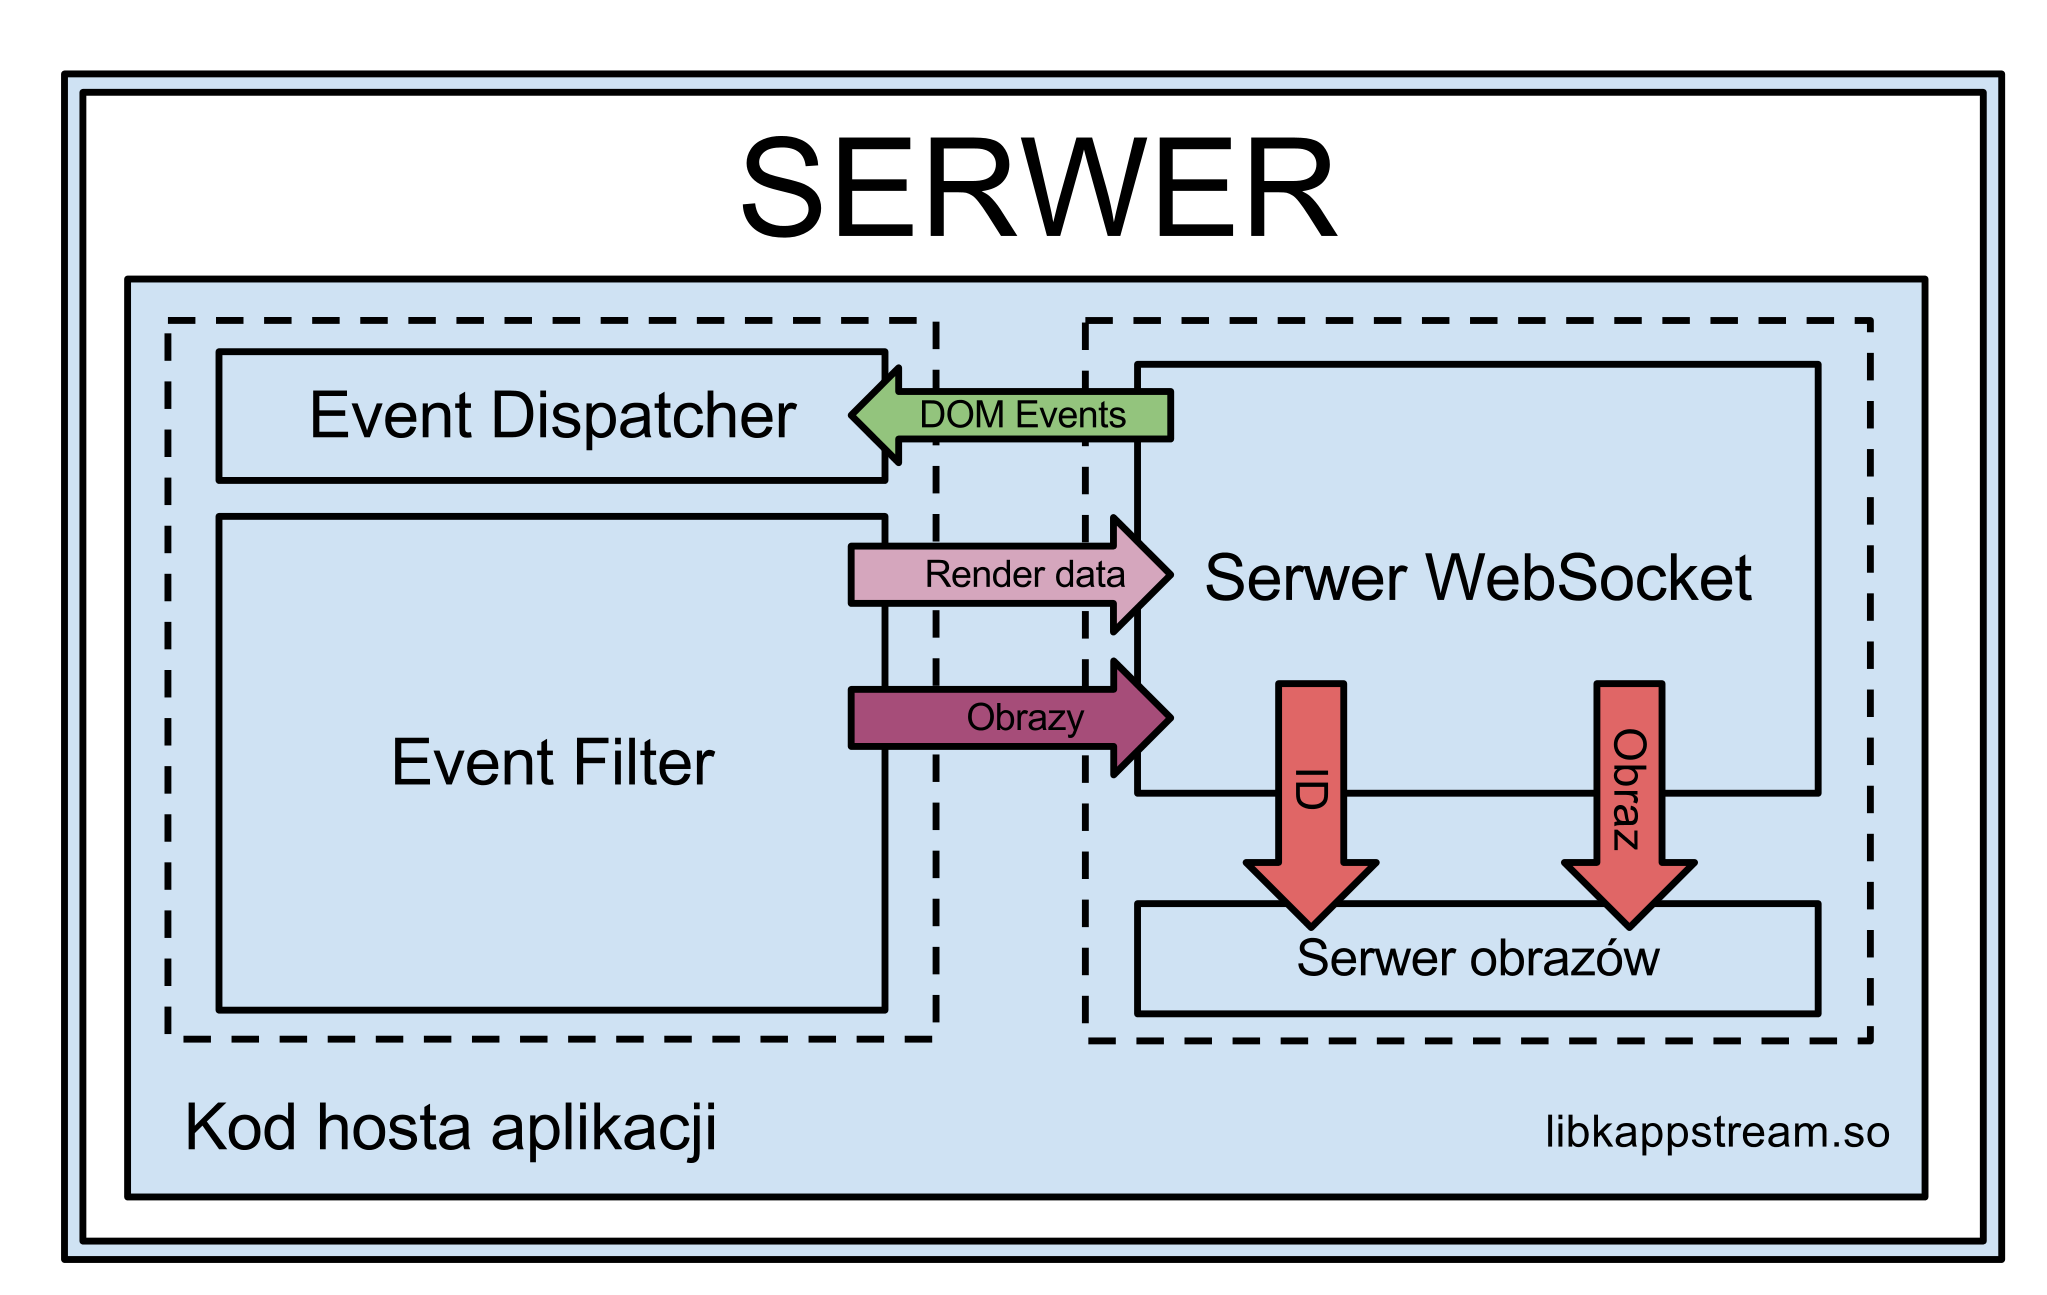
\includegraphics[width=0.8\linewidth]{img/arch-lib}
\caption{Schemat wewnętrznych przepływów danych w module WebSocket.}
\label{fig:arch-lib}
\end{figure}
